\chapter{Methods}
\index{Methods@\emph{Methods}}%
\section{Phonetics of Metrics in Estonian Word Prosody}

Primary lexical stress in native Estonian words is fixed, falling on word-initial syllables. There are no stress minimal pairs at the lexical level: thus, primary stress is said to be {\it demarcative} or {\it identificational}\citep{lehiste1992}, functioning to indicate the boundary of a new word. Syllables following primary stress are unstressed, and secondary stress is attested to fall on each odd syllable in polysyllabic words. Duration functions at several levels of Estonian prosody: it is the strongest correlate of both clear speech and stress \citep{lippusAsuMari2014} when compared with measurements of f0 and spectral emphasis, and is independently contrastive at the segmental level as illustrated in minimal triads in \ref{qperm}. Secondary stress was found to be significantly different in duration from both primary and peninitial unstressed syllables: interestingly, secondary stressed syllables were not shown to differ greatly from their even-positioned neighbors (excepting the peninitial). For the sake of simplicity, this study focuses only on the contrast between first (primary stressed) and second (unstressed) syllables. 

%\cite{eekmeisterUralica98}

In primary stress position, there are three contrastive syllable quantities. The first (Q1) is described as short, the next (Q2) as long, and the heaviest (Q3) as overlong. 

%This ternary contrast has long been the subject of debate in the phonological literature of metrics: Q3 syllables have been analyzed both as a monosyllabic foot \citep{princeMetricalTheoryEstonian1980} and as a trimoraic syllable \citep{hayesCompensatoryLengtheningMoraic1989, kuznetsovaEstonianWordProsody2018,prillopMoraeEstonianReply2020}. 


 \begin{table}[htb]
\centering
\begin{tabular}{ccc}
\hline
Q1 & Q2 & Q3 \\
{\it kodi	} 	& {\it koodi }	& {\it koodi }	\\  
/ko.ti/		& /koː.ti/	& /koːː.ti/	\\
\hline
		& {\it koti }	& {\it kotti}	 \\
		& /kot.ti/	& /kotː.ti/	\\
\hline
		& {\it gooti}	& {\it kooti} 	\\
		& /koːt.ti/	& /koːːt.ti/	\\
\hline
\end{tabular}
\label{qperm}
\caption{segmental permutations of initial syllable quantity}
\end{table}

In the first row of \ref{qperm}, we see a minimal triad of the ternary quantity contrast in open first syllables. The Q2 and Q3 columns demonstrate all the other ways this contrast can be realized using the same segment identities in closed syllables. 

\begin{exe}
\ex \gll laul-da \\
	{[ˈlɑuːl.dɑ]} \\
	sing-\Tr{} 
	\glt	`singing'
\ex 	ööbik \\
	{[ˈøː.pikː]} \\
	nightingale.\Nom{} 
	\glt`nightingale'
\label{disyllables}
\end{exe}
Q1 and Q2 syllables can be both stressed and unstressed, while Q3 is only present in stressed positions, attracting stress to its (non-initial) syllable in compound and loan words. Peninitial syllables can only be Q1 or Q2, illustrated in \ref{disyllables}. 


\section{Constructing the Corpus}

I first describe the source materials and the selection criteria for the sample corpus of {\it regilaul} folksongs. Following this, the annotation and measurement procedure is detailed. Then the procedure for assembling the corpus of songs and their text annotations is covered before proceeding to the inclusion criteria for vowel duration and dispersion measurements.

\subsection{Materials}



%Until 1948, songs were collected on wax cylinders, then played on a phonograph and transcribed. shellac discs 1936-38, 746 recordings, 
%analogue is the biggest collection in the archive, with over 80,000 individual recordings. Open-reel tape, cassette recordings since the 1970s. 
%both wax and disc were re-recorded onto open-reel tape in 78-79.
%Presently, the sound engineer Jaan Tamm has been working on preserving the earlier tape recordings in digital form for the EFA. WAV files are stored on CD-Rom at the EFA in Tartu, Estonia, while .mp3 and .ogg lossy formats are uploaded to the internet database. 
% collected by Herbert Tampere, Erna Tampere, and Ottilie Kõiva between 1912 and 1966 for the Estonian Folklore Archives in Tartu, Estonia. \\
%
% and   tunes
%the total number of song recordings is over 26,000. Of these, over 11,000 are from the beginning of the 20th century. Tampere did like 2,000 of them..
%
%%
%The need for writing the tunes live during fieldwork has reduced with the availability of analog and now digital audio recording equipment.




Songs for this paper were accessed via The Anthology of Estonian Traditional Music \citep{tampere2016}. Originally published on four vinyl discs in 1970, the digital version showcases a robust sample of the massive collection of {\it regilaul} in Estonian Folklore Archives. In addition to audio, the  compilation includes  photographs, sheet music, and performer demographics of 98 {\it regilaul} songs and 17 instrumental tunes. 
These songs were compiled in part by Herbert Tampere, an early ethnomusicology field work organizer of the EFA, who along with Erna Tampere and Ottilie Kõiva collected these folk songs\citep{oras2002, tampere2016}. 
% Pictured in \ref{tampy} is a photograph taken of one of the very field trips to record songs studied in this paper. 
%
%\begin{figure}[htb]
%\centering
%
%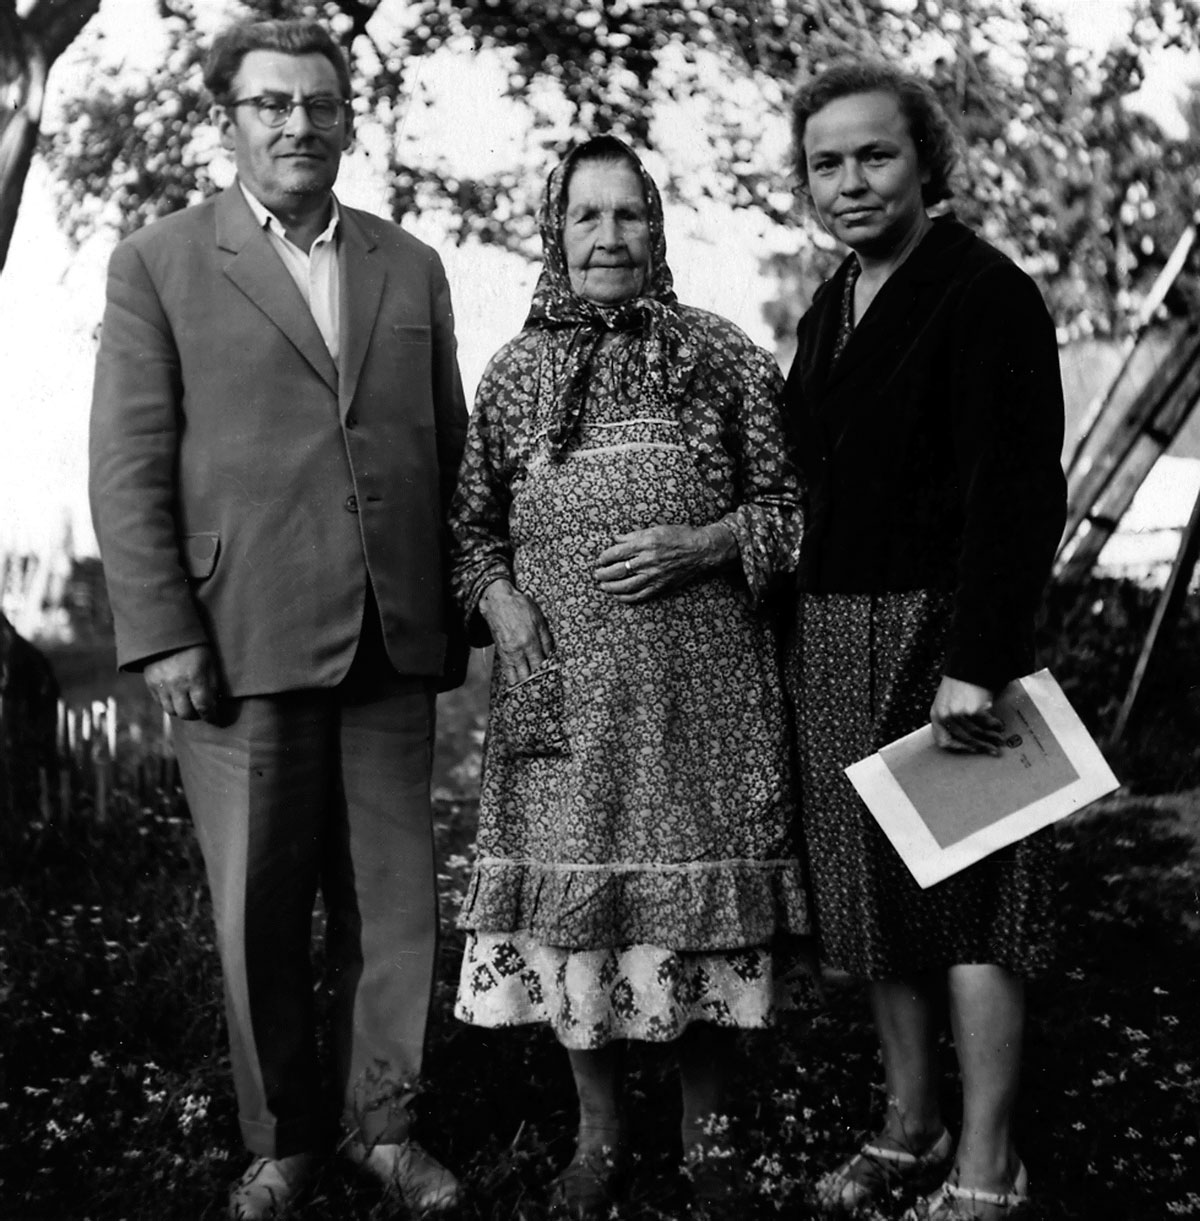
\includegraphics[width=200pt]{figures/Mf_07027_Tampered_Orik.jpg}
%\caption{Herbert Tampere on a field trip}
%\label{tampy}
%\end{figure}


While the ultimate goal is to continue annotation of the entire available corpus of {\it regilaul}, for the initial analysis I chose a sample of songs all belonging to the same regional dialect and recording method. Once several regions were identified as possible candidates, a native Estonian speaker was consulted on the final selection. The nine songs analyzed in this study were all recorded in Parnümaa county from 1961-1966 by Herbert and Erna Tampere. 
% The first criteria is due to the lossy nature of some of the older files available on the site: the online versions are all compressed lossy, so the analog audio originally recorded on tape and then digitized have a higher resolution, even compressed, than songs that have been copied from wax cylinders or shellac discs onto open-reel tape and then digitizing. 


\section{Annotating the Song Audio }

 Each song's lyrics are copied from the site and saved as .txt files in Estonian orthography, each line of the file corresponding to one melody line.  
Audio files of the selected songs are downloaded from the archive in .ogg format, which is the highest resolution of the two lossy formats available from the digital anthology. Each song is then imported into a Logic Pro X \citep{logic2014} session for beat detection, tempo mapping, and trimming. 
To make the tempo map, the session must be set to {\it flex tempo}. From here a beat onset detection algorithm is  given the transcribed bpm and time signature from the archived song data and run on the imported audio file. The result is an annotation of intervals in time, and the bpm for each measure is annotated according to the performance of the song.
The tempo map allows us to document when {\it exactly} in time the particular singer performed a given note, the duration of the sung note, and the acoustic threshold by which the note is defined as ``strong" relative to surrounding notes. The process is informed by the transcribed bpm and time signature included in the anthology. This is beneficial to my purposes in two ways: by accounting for the natural tempo variation in live performance, and by using a consistent metric to determine beat strength acoustically rather than just perceptually. Using onset detection algorithms such as these \citep{bKeeper2007} in phonetics research, especially in the interdisciplinary field of linguistics and musicology, will be particularly beneficial to answering questions about rhythm: finding a way to bring our intuitions and impressions about ``the beat" together with the acoustic phenomenon. By automating the annotation and measurement process using open source tools, the author hopes to share these machines with those who have similar research interests, and also to invite contributors to the data of this corpus of text data time-aligned to queryable audio signal data. From here, a MIDI track is programmed to create a metronome that is the length of a single syllable-note in the song. In most of these, a 4/4 measure contains eight eighth notes, so the metronome track contains four eighth notes indicating the ``ictus" beats. In flex tempo mode, the MIDI track adjusts note and measure length to match the fluctuations in tempo as documented in the map for the song. The metronome and the song audio file are trimmed to match exactly, and the metronome is converted into a textgrid in PRAAT\citep{boersna2022}, where the annotation process continues. 

 
The orthographic text phrases of the song lyrics are then inserted into each phrase interval with a script, and then eSpeak forced aligner for Estonian \citep{eSpeak1995} is run on each phrase to the word and phonemic level. Because this forced aligner is trained on spoken, not sung Estonian, the aligner sometimes tries to align words into the signal before they are uttered. In these cases, the word level tier is manually realigned so that it contains all and only the transcribed word, and then the forced aligner is re-run on this word to the segmental level. ``Giving" the forced-aligner all and only the correct word improved the segmental alignment, but the relevant segments for this study were manually verified and adjusted (if necessary) to ensure they all met a consistent criteria. 
\subsection{Criteria for adjusting the forced-aligner}


Manually verified the intervals set by the forced aligner for syllable nuclei according to the frequency and intensity contours in PRAAT. 
The beginning of the vowel was broadly aligned according to a combination of acoustic correlates: at the point where 1. intensity was within 2dB of the steady-state medial portion of the vowel with a slope between 0.5 and zero, 2. frequency stabilizing into that syllable-note's pitch category, and 3. the presence of a voicing bar and visible formants f1, f2, and f3. Manner specific criteria: did not include burst in plosives. Boundaries between fricative onsets and vowels was determined by the end of visible high-frequency noise in the spectrum. Coronal fricative /s/ also consistently showed a carat \ref{} in the frequency track immediately preceding the transition to vowel. For approximants, the additional criteria of steady formants was necessary. Following nasal onsets, vowel intensity {\it lowered}, but a near-zero slope still reliably coincided with the other acoustic correlates. 


 The offset boundaries of vowels was set similarly, but instead with slopes less than or equal to -1 in their transition to occlusions. The first three formants were more variable in transition to codas, so the other cues were relied on more heavily. 

Closed syllables with approximant codas /l/were excluded, as neither the forced-aligner nor the phonetician could determine a reliable way to define the boundary between them. In onset position, the boundary between approximant and vowel was more consistently definable by the above criteria (with the additional requirement of steady formants, which generally coincided with the frequency and intensity cues). In cases of vowel adjacency across syllable boundaries, the presence of a visible glottal stop and a similar (though not as strict) pattern to the above criteria would qualify both for inclusion. In the absence of these cues, both nuclei were excluded from the measurements. Other exclusions were due to ambient noise (i.e., churchbells in song 41), ambiguity of word boundaries due to wordplay or nonse words (verified by native speaker informant), and cases where the transcription indicated epenthesis or severe reduction. 
%epenthesized vowels (i.e., pandi mind paju raiumaie) having mind(e) \\


In all cases, if the aforementioned cues were unavailable, ambiguous, or misaligned, the token was elided for this analysis. From all nine songs in the corpus, a total of 757 vowel nuclei met the criteria for inclusion in duration measurements. 


At this point, the audio recording of each song has tiers annotated for tempo and strong beat, verse line phrases, two interval tiers force-aligned to word and phoneme levels, and a separate tier with intervals of the individual vowel segments of interest copied from the phoneme tier.
\subsection{Fusing audio-aligned transcriptions with text corpus}

The last step in preprocessing is to integrate the annotation of the song audio with the lexical content of the song. This study accomplishes the task using an open-source natural language toolkit in python called estinltk \url{https://github.com/estnltk} \citep{estnltk2020}. Among other things, the toolkit has a robust dictionary of Estonian grammar, including phonetic transcription of syllables with corresponding quantity and stress data. 


Thus the data structure of this corpus offers two independent metrics of rhythmic prominence in these songs. From the audio recording and the beat detection, we have an annotation of strong beats based on replicable acoustic measurements, and from the dictionary in the natural language toolkit, we have native speaker intuitions about the lexical weight and prominence in the words of the text. While the stress system is generally predictable, the syllable quantity is not always apparent from the orthography, and not always detectible by a non-native listener. 
%Linguistic descriptions of the Estonian language date back as early as the seventeenth century, but the ternary quantity contrast was not documented until native Estonian linguists contributed their intuitions. The non-native linguists had only described lexical stress \citep{sargEarlyHistoryEstonian2005a}. \\



Once the annotations are complete, the corresponding text files are aggregated and, the corresponding measurements from PRAAT are concatenated via python using the parselmouth library python interface to PRAAT \citep{parselmouth2018, python1995}. 

Only those vowels from syllables that were nominally transcribed as isochronous eighth notes and also coincided with the beat length provided by the flexible MIDI metronome were used for this study.  Syllables in the final position of the verse were excluded due to the tendency for variation in the final notes of the phrase. 
%Each verse line is considered a ``semantic rhyme" \citep{lehiste1978}, or a meaningfully complete constituent. 
\subsection{long vowels and monophthongs}
An estonian word game supports the notion of many-to-one phonemes for long vowels, but a one-to-one status for diphthongs.

\begin{exe}

\ex  long vowels (Q1,Q2, Q3 contrast) 
	\begin{itemize} 
	\item sada `hundred' $\rightarrow$ sapida 
	\item  saada `send' (2nd sg. imp.) $\rightarrow$ sapiida (*sapiada)(*saapida)
	\item saada `get' , {\it -da} infinitive $\rightarrow$ sapii:da (*sapiada)(*saapida)
	\end{itemize}
\ex 	 diphthongs \\
laulus `in the song' (iness.sg) $\rightarrow$ lapiulus (*laupilus)
\end{exe}

In both cases, `pi' carries the prosodic characteristics of the displaced syllable. the stress is moved from first syllable to 'pi,' and also the length. crucially, the diphthong is split at the segmental level, while the long vowels are not.  Long vowels, then, are treated as monophonematic, whereas diphthongs are treated as biphonematic. 

This word game supports the notion that long (identical) vowels and diphthongs in  Estonian should potentially be treated as different categories for duration. The analysis therefore will examine long monophthongs and diphthongs both together and separately for interpreting  the measurement of vowel duration. 

\cite{lehiste1985}

\subsection{Statistical Analysis} 
%Linear mixed-effects model using lme4 in R \cite{rlme4}. 
%
%For stress and ictus, only q1 and q2 syllables (Q3 never unstressed). \\
%for quantity and ictus, only word-level stressed syllables
%
%
%
%Design-based formula
%Hierarchical Linear Model with group-specific terms
%
%\cite{goodrichRstanarmBayesianApplied2020,brillemanJointLongitudinalTimetoevent2018}
